% Options for packages loaded elsewhere
\PassOptionsToPackage{unicode}{hyperref}
\PassOptionsToPackage{hyphens}{url}
\PassOptionsToPackage{dvipsnames,svgnames,x11names}{xcolor}
%
\documentclass[
  letterpaper,
  DIV=11,
  numbers=noendperiod]{scrartcl}

\usepackage{amsmath,amssymb}
\usepackage{iftex}
\ifPDFTeX
  \usepackage[T1]{fontenc}
  \usepackage[utf8]{inputenc}
  \usepackage{textcomp} % provide euro and other symbols
\else % if luatex or xetex
  \usepackage{unicode-math}
  \defaultfontfeatures{Scale=MatchLowercase}
  \defaultfontfeatures[\rmfamily]{Ligatures=TeX,Scale=1}
\fi
\usepackage{lmodern}
\ifPDFTeX\else  
    % xetex/luatex font selection
\fi
% Use upquote if available, for straight quotes in verbatim environments
\IfFileExists{upquote.sty}{\usepackage{upquote}}{}
\IfFileExists{microtype.sty}{% use microtype if available
  \usepackage[]{microtype}
  \UseMicrotypeSet[protrusion]{basicmath} % disable protrusion for tt fonts
}{}
\makeatletter
\@ifundefined{KOMAClassName}{% if non-KOMA class
  \IfFileExists{parskip.sty}{%
    \usepackage{parskip}
  }{% else
    \setlength{\parindent}{0pt}
    \setlength{\parskip}{6pt plus 2pt minus 1pt}}
}{% if KOMA class
  \KOMAoptions{parskip=half}}
\makeatother
\usepackage{xcolor}
\setlength{\emergencystretch}{3em} % prevent overfull lines
\setcounter{secnumdepth}{-\maxdimen} % remove section numbering
% Make \paragraph and \subparagraph free-standing
\makeatletter
\ifx\paragraph\undefined\else
  \let\oldparagraph\paragraph
  \renewcommand{\paragraph}{
    \@ifstar
      \xxxParagraphStar
      \xxxParagraphNoStar
  }
  \newcommand{\xxxParagraphStar}[1]{\oldparagraph*{#1}\mbox{}}
  \newcommand{\xxxParagraphNoStar}[1]{\oldparagraph{#1}\mbox{}}
\fi
\ifx\subparagraph\undefined\else
  \let\oldsubparagraph\subparagraph
  \renewcommand{\subparagraph}{
    \@ifstar
      \xxxSubParagraphStar
      \xxxSubParagraphNoStar
  }
  \newcommand{\xxxSubParagraphStar}[1]{\oldsubparagraph*{#1}\mbox{}}
  \newcommand{\xxxSubParagraphNoStar}[1]{\oldsubparagraph{#1}\mbox{}}
\fi
\makeatother

\usepackage{color}
\usepackage{fancyvrb}
\newcommand{\VerbBar}{|}
\newcommand{\VERB}{\Verb[commandchars=\\\{\}]}
\DefineVerbatimEnvironment{Highlighting}{Verbatim}{commandchars=\\\{\}}
% Add ',fontsize=\small' for more characters per line
\usepackage{framed}
\definecolor{shadecolor}{RGB}{241,243,245}
\newenvironment{Shaded}{\begin{snugshade}}{\end{snugshade}}
\newcommand{\AlertTok}[1]{\textcolor[rgb]{0.68,0.00,0.00}{#1}}
\newcommand{\AnnotationTok}[1]{\textcolor[rgb]{0.37,0.37,0.37}{#1}}
\newcommand{\AttributeTok}[1]{\textcolor[rgb]{0.40,0.45,0.13}{#1}}
\newcommand{\BaseNTok}[1]{\textcolor[rgb]{0.68,0.00,0.00}{#1}}
\newcommand{\BuiltInTok}[1]{\textcolor[rgb]{0.00,0.23,0.31}{#1}}
\newcommand{\CharTok}[1]{\textcolor[rgb]{0.13,0.47,0.30}{#1}}
\newcommand{\CommentTok}[1]{\textcolor[rgb]{0.37,0.37,0.37}{#1}}
\newcommand{\CommentVarTok}[1]{\textcolor[rgb]{0.37,0.37,0.37}{\textit{#1}}}
\newcommand{\ConstantTok}[1]{\textcolor[rgb]{0.56,0.35,0.01}{#1}}
\newcommand{\ControlFlowTok}[1]{\textcolor[rgb]{0.00,0.23,0.31}{\textbf{#1}}}
\newcommand{\DataTypeTok}[1]{\textcolor[rgb]{0.68,0.00,0.00}{#1}}
\newcommand{\DecValTok}[1]{\textcolor[rgb]{0.68,0.00,0.00}{#1}}
\newcommand{\DocumentationTok}[1]{\textcolor[rgb]{0.37,0.37,0.37}{\textit{#1}}}
\newcommand{\ErrorTok}[1]{\textcolor[rgb]{0.68,0.00,0.00}{#1}}
\newcommand{\ExtensionTok}[1]{\textcolor[rgb]{0.00,0.23,0.31}{#1}}
\newcommand{\FloatTok}[1]{\textcolor[rgb]{0.68,0.00,0.00}{#1}}
\newcommand{\FunctionTok}[1]{\textcolor[rgb]{0.28,0.35,0.67}{#1}}
\newcommand{\ImportTok}[1]{\textcolor[rgb]{0.00,0.46,0.62}{#1}}
\newcommand{\InformationTok}[1]{\textcolor[rgb]{0.37,0.37,0.37}{#1}}
\newcommand{\KeywordTok}[1]{\textcolor[rgb]{0.00,0.23,0.31}{\textbf{#1}}}
\newcommand{\NormalTok}[1]{\textcolor[rgb]{0.00,0.23,0.31}{#1}}
\newcommand{\OperatorTok}[1]{\textcolor[rgb]{0.37,0.37,0.37}{#1}}
\newcommand{\OtherTok}[1]{\textcolor[rgb]{0.00,0.23,0.31}{#1}}
\newcommand{\PreprocessorTok}[1]{\textcolor[rgb]{0.68,0.00,0.00}{#1}}
\newcommand{\RegionMarkerTok}[1]{\textcolor[rgb]{0.00,0.23,0.31}{#1}}
\newcommand{\SpecialCharTok}[1]{\textcolor[rgb]{0.37,0.37,0.37}{#1}}
\newcommand{\SpecialStringTok}[1]{\textcolor[rgb]{0.13,0.47,0.30}{#1}}
\newcommand{\StringTok}[1]{\textcolor[rgb]{0.13,0.47,0.30}{#1}}
\newcommand{\VariableTok}[1]{\textcolor[rgb]{0.07,0.07,0.07}{#1}}
\newcommand{\VerbatimStringTok}[1]{\textcolor[rgb]{0.13,0.47,0.30}{#1}}
\newcommand{\WarningTok}[1]{\textcolor[rgb]{0.37,0.37,0.37}{\textit{#1}}}

\providecommand{\tightlist}{%
  \setlength{\itemsep}{0pt}\setlength{\parskip}{0pt}}\usepackage{longtable,booktabs,array}
\usepackage{calc} % for calculating minipage widths
% Correct order of tables after \paragraph or \subparagraph
\usepackage{etoolbox}
\makeatletter
\patchcmd\longtable{\par}{\if@noskipsec\mbox{}\fi\par}{}{}
\makeatother
% Allow footnotes in longtable head/foot
\IfFileExists{footnotehyper.sty}{\usepackage{footnotehyper}}{\usepackage{footnote}}
\makesavenoteenv{longtable}
\usepackage{graphicx}
\makeatletter
\def\maxwidth{\ifdim\Gin@nat@width>\linewidth\linewidth\else\Gin@nat@width\fi}
\def\maxheight{\ifdim\Gin@nat@height>\textheight\textheight\else\Gin@nat@height\fi}
\makeatother
% Scale images if necessary, so that they will not overflow the page
% margins by default, and it is still possible to overwrite the defaults
% using explicit options in \includegraphics[width, height, ...]{}
\setkeys{Gin}{width=\maxwidth,height=\maxheight,keepaspectratio}
% Set default figure placement to htbp
\makeatletter
\def\fps@figure{htbp}
\makeatother

\KOMAoption{captions}{tableheading}
\makeatletter
\@ifpackageloaded{caption}{}{\usepackage{caption}}
\AtBeginDocument{%
\ifdefined\contentsname
  \renewcommand*\contentsname{Table of contents}
\else
  \newcommand\contentsname{Table of contents}
\fi
\ifdefined\listfigurename
  \renewcommand*\listfigurename{List of Figures}
\else
  \newcommand\listfigurename{List of Figures}
\fi
\ifdefined\listtablename
  \renewcommand*\listtablename{List of Tables}
\else
  \newcommand\listtablename{List of Tables}
\fi
\ifdefined\figurename
  \renewcommand*\figurename{Figure}
\else
  \newcommand\figurename{Figure}
\fi
\ifdefined\tablename
  \renewcommand*\tablename{Table}
\else
  \newcommand\tablename{Table}
\fi
}
\@ifpackageloaded{float}{}{\usepackage{float}}
\floatstyle{ruled}
\@ifundefined{c@chapter}{\newfloat{codelisting}{h}{lop}}{\newfloat{codelisting}{h}{lop}[chapter]}
\floatname{codelisting}{Listing}
\newcommand*\listoflistings{\listof{codelisting}{List of Listings}}
\makeatother
\makeatletter
\makeatother
\makeatletter
\@ifpackageloaded{caption}{}{\usepackage{caption}}
\@ifpackageloaded{subcaption}{}{\usepackage{subcaption}}
\makeatother

\ifLuaTeX
  \usepackage{selnolig}  % disable illegal ligatures
\fi
\usepackage{bookmark}

\IfFileExists{xurl.sty}{\usepackage{xurl}}{} % add URL line breaks if available
\urlstyle{same} % disable monospaced font for URLs
\hypersetup{
  pdftitle={Class 05: Data Visualization with GGPLOT},
  pdfauthor={Mia Fava},
  colorlinks=true,
  linkcolor={blue},
  filecolor={Maroon},
  citecolor={Blue},
  urlcolor={Blue},
  pdfcreator={LaTeX via pandoc}}


\title{Class 05: Data Visualization with GGPLOT}
\author{Mia Fava}
\date{}

\begin{document}
\maketitle


\subsection{Plotting in R}\label{plotting-in-r}

R has lot's of ways to make plots and figures. This includes so-called
\textbf{base} graphics and packages like \textbf{ggplot2}

\begin{Shaded}
\begin{Highlighting}[]
\FunctionTok{plot}\NormalTok{(cars)}
\end{Highlighting}
\end{Shaded}

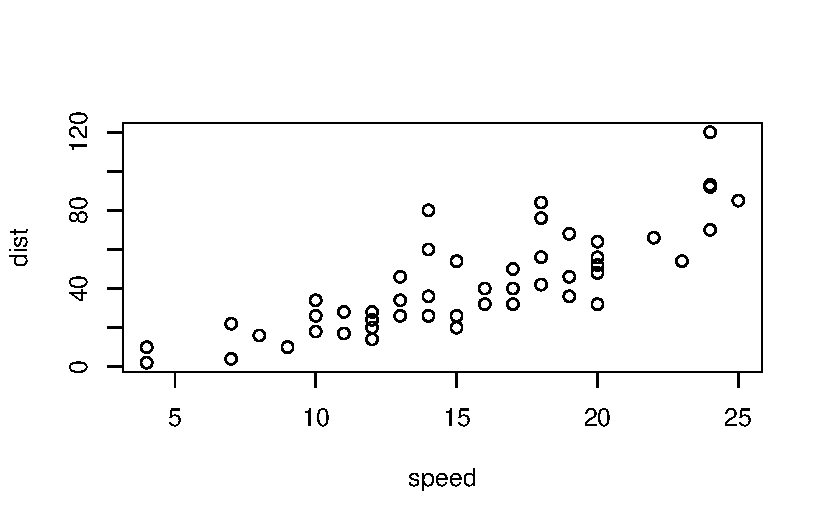
\includegraphics{class05_files/figure-pdf/unnamed-chunk-1-1.pdf}

This is a \textbf{base} R plot of the in-built \texttt{cars} dataset
that has only two columns:

\begin{Shaded}
\begin{Highlighting}[]
\NormalTok{cars}
\end{Highlighting}
\end{Shaded}

\begin{verbatim}
   speed dist
1      4    2
2      4   10
3      7    4
4      7   22
5      8   16
6      9   10
7     10   18
8     10   26
9     10   34
10    11   17
11    11   28
12    12   14
13    12   20
14    12   24
15    12   28
16    13   26
17    13   34
18    13   34
19    13   46
20    14   26
21    14   36
22    14   60
23    14   80
24    15   20
25    15   26
26    15   54
27    16   32
28    16   40
29    17   32
30    17   40
31    17   50
32    18   42
33    18   56
34    18   76
35    18   84
36    19   36
37    19   46
38    19   68
39    20   32
40    20   48
41    20   52
42    20   56
43    20   64
44    22   66
45    23   54
46    24   70
47    24   92
48    24   93
49    24  120
50    25   85
\end{verbatim}

\begin{quote}
Q. How would we plot this wee dataset with \textbf{ggplot2}?
\end{quote}

All ggplot figures have at least 3 layers:

-\textbf{data} -\textbf{aes} (how data map to the plot) -\textbf{geoms}
(how we draw the plot, lines, points, etc)

Before I use any new packages I need to download and install it with the
\texttt{install.packages()} command.

I never use \texttt{install.packages()} within my quarto document
otherwise I will install the package over and over and over again, which
is silly!

Once a package is installed I can load it up with the
\texttt{libraary()} function

\begin{Shaded}
\begin{Highlighting}[]
\CommentTok{\# install.packages("ggplot2")}
\FunctionTok{library}\NormalTok{(ggplot2)}
\FunctionTok{ggplot}\NormalTok{(cars) }\SpecialCharTok{+} 
  \FunctionTok{aes}\NormalTok{(}\AttributeTok{x=}\NormalTok{speed, }\AttributeTok{y=}\NormalTok{dist) }\SpecialCharTok{+}
  \FunctionTok{geom\_point}\NormalTok{()}
\end{Highlighting}
\end{Shaded}

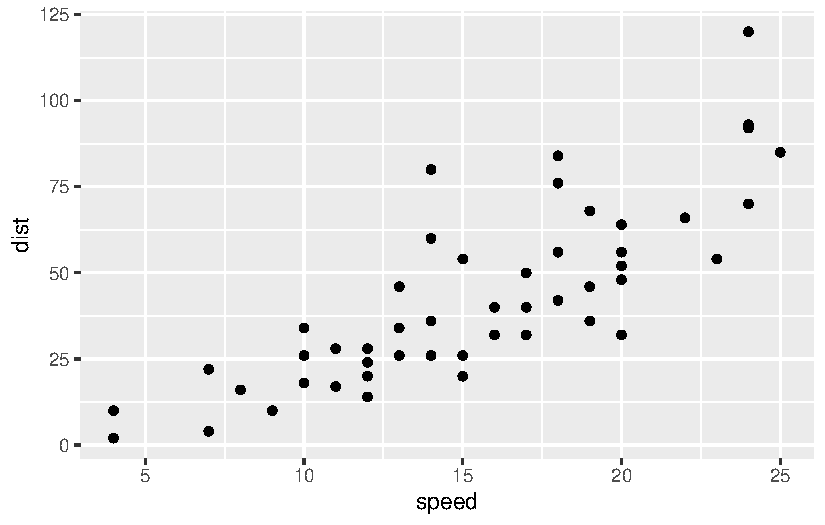
\includegraphics{class05_files/figure-pdf/unnamed-chunk-3-1.pdf}

Key point: For simple plots (like the one above) ggplot is more verbose
(we need to do more typing) but as plots get more complicated ggplot
starts to be more clear and simple than base R plot()

\begin{Shaded}
\begin{Highlighting}[]
\FunctionTok{ggplot}\NormalTok{(cars) }\SpecialCharTok{+}
  \FunctionTok{aes}\NormalTok{(}\AttributeTok{x=}\NormalTok{speed, }\AttributeTok{y=}\NormalTok{dist) }\SpecialCharTok{+}
  \FunctionTok{geom\_point}\NormalTok{() }\SpecialCharTok{+} 
  \FunctionTok{geom\_smooth}\NormalTok{(}\AttributeTok{method=}\StringTok{"lm"}\NormalTok{,}\AttributeTok{se =} \ConstantTok{FALSE}\NormalTok{ ) }\SpecialCharTok{+}
  \FunctionTok{labs}\NormalTok{(}\AttributeTok{title=}\StringTok{"Stopping distance of old cars"}\NormalTok{, }\AttributeTok{x=}\StringTok{"Speed (MPH)"}\NormalTok{, }\AttributeTok{y=}\StringTok{"Stopping distance (ft)"}\NormalTok{, }\AttributeTok{subtitle =} \StringTok{"From the in{-}built cars dataset"}\NormalTok{, }\AttributeTok{caption=}\StringTok{"Dataset: \textquotesingle{}cars\textquotesingle{}"}\NormalTok{) }\SpecialCharTok{+}
  \FunctionTok{theme\_bw}\NormalTok{()}
\end{Highlighting}
\end{Shaded}

\begin{verbatim}
`geom_smooth()` using formula = 'y ~ x'
\end{verbatim}

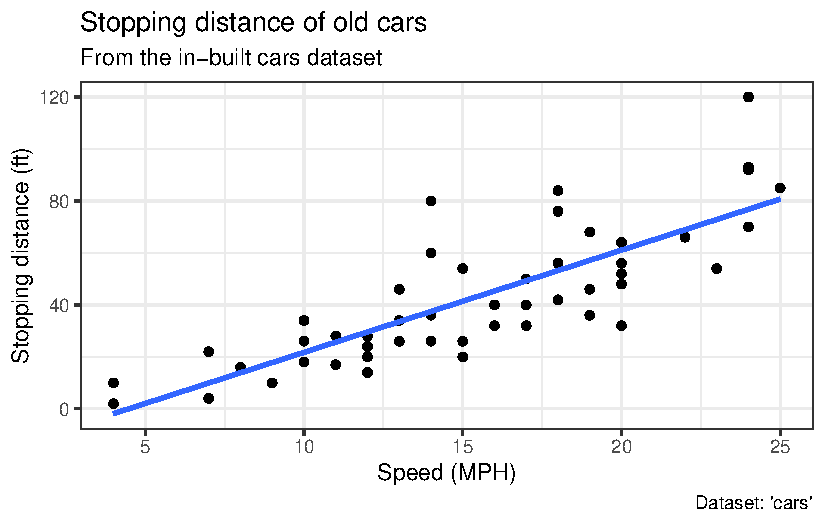
\includegraphics{class05_files/figure-pdf/unnamed-chunk-4-1.pdf}

\begin{Shaded}
\begin{Highlighting}[]
\NormalTok{url }\OtherTok{\textless{}{-}} \StringTok{"https://bioboot.github.io/bimm143\_S20/class{-}material/up\_down\_expression.txt"}
\NormalTok{genes }\OtherTok{\textless{}{-}} \FunctionTok{read.delim}\NormalTok{(url)}
\FunctionTok{head}\NormalTok{(genes)}
\end{Highlighting}
\end{Shaded}

\begin{verbatim}
        Gene Condition1 Condition2      State
1      A4GNT -3.6808610 -3.4401355 unchanging
2       AAAS  4.5479580  4.3864126 unchanging
3      AASDH  3.7190695  3.4787276 unchanging
4       AATF  5.0784720  5.0151916 unchanging
5       AATK  0.4711421  0.5598642 unchanging
6 AB015752.4 -3.6808610 -3.5921390 unchanging
\end{verbatim}

\begin{Shaded}
\begin{Highlighting}[]
\FunctionTok{nrow}\NormalTok{(genes)}
\end{Highlighting}
\end{Shaded}

\begin{verbatim}
[1] 5196
\end{verbatim}

\begin{Shaded}
\begin{Highlighting}[]
\FunctionTok{colnames}\NormalTok{(genes)}
\end{Highlighting}
\end{Shaded}

\begin{verbatim}
[1] "Gene"       "Condition1" "Condition2" "State"     
\end{verbatim}

\begin{Shaded}
\begin{Highlighting}[]
\FunctionTok{table}\NormalTok{(genes}\SpecialCharTok{$}\NormalTok{State)}
\end{Highlighting}
\end{Shaded}

\begin{verbatim}

      down unchanging         up 
        72       4997        127 
\end{verbatim}

\begin{Shaded}
\begin{Highlighting}[]
\FunctionTok{round}\NormalTok{( }\FunctionTok{table}\NormalTok{(genes}\SpecialCharTok{$}\NormalTok{State)}\SpecialCharTok{/}\FunctionTok{nrow}\NormalTok{(genes) }\SpecialCharTok{*} \DecValTok{100}\NormalTok{,}\DecValTok{2}\NormalTok{)}
\end{Highlighting}
\end{Shaded}

\begin{verbatim}

      down unchanging         up 
      1.39      96.17       2.44 
\end{verbatim}

The key functions here were: \texttt{nrow()} and \texttt{ncol()}
\texttt{table()} is very useful for getting counts finally
\texttt{round()}

A first plot:

\begin{Shaded}
\begin{Highlighting}[]
\FunctionTok{ggplot}\NormalTok{(genes) }\SpecialCharTok{+} 
    \FunctionTok{aes}\NormalTok{(}\AttributeTok{x=}\NormalTok{Condition1, }\AttributeTok{y=}\NormalTok{Condition2) }\SpecialCharTok{+}
    \FunctionTok{geom\_point}\NormalTok{() }
\end{Highlighting}
\end{Shaded}

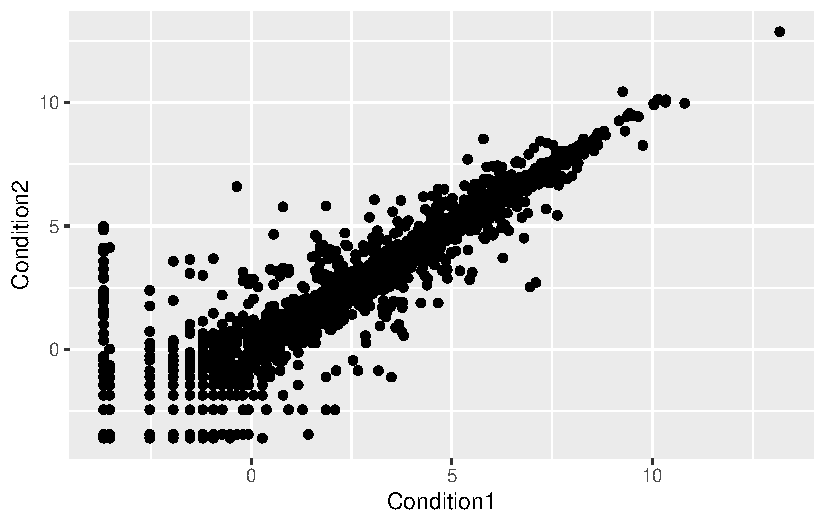
\includegraphics{class05_files/figure-pdf/unnamed-chunk-6-1.pdf}

A Second Plot:

\begin{Shaded}
\begin{Highlighting}[]
\FunctionTok{ggplot}\NormalTok{(genes) }\SpecialCharTok{+} 
    \FunctionTok{aes}\NormalTok{(}\AttributeTok{x=}\NormalTok{Condition1, }\AttributeTok{y=}\NormalTok{Condition2, }\AttributeTok{col=}\NormalTok{State) }\SpecialCharTok{+}
    \FunctionTok{geom\_point}\NormalTok{() }
\end{Highlighting}
\end{Shaded}

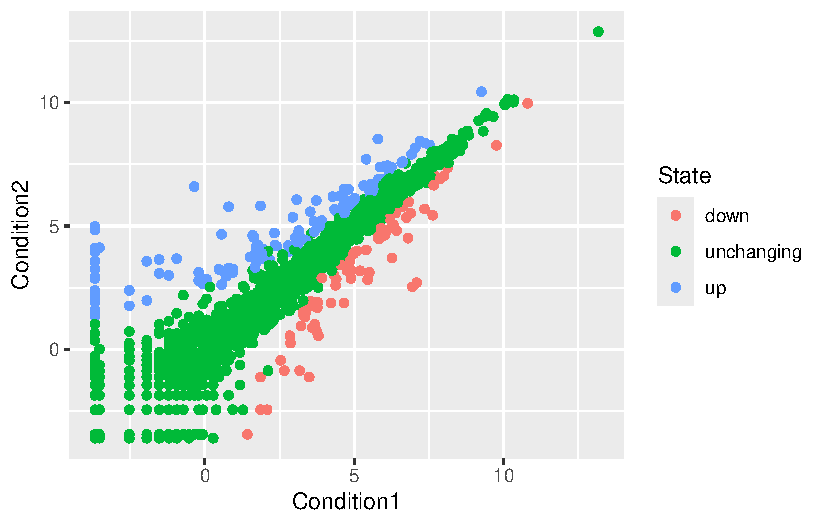
\includegraphics{class05_files/figure-pdf/unnamed-chunk-7-1.pdf}

Change the color

A Third Plot:

\begin{Shaded}
\begin{Highlighting}[]
\FunctionTok{ggplot}\NormalTok{(genes) }\SpecialCharTok{+} 
    \FunctionTok{aes}\NormalTok{(}\AttributeTok{x=}\NormalTok{Condition1, }\AttributeTok{y=}\NormalTok{Condition2, }\AttributeTok{col=}\NormalTok{State) }\SpecialCharTok{+}
    \FunctionTok{geom\_point}\NormalTok{()}\SpecialCharTok{+}
\FunctionTok{scale\_colour\_manual}\NormalTok{(}\AttributeTok{values=}\FunctionTok{c}\NormalTok{(}\StringTok{"blue"}\NormalTok{,}\StringTok{"gray"}\NormalTok{,}\StringTok{"red"}\NormalTok{)) }\SpecialCharTok{+}
    \FunctionTok{labs}\NormalTok{(}\AttributeTok{title=}\StringTok{"Gene Expresion Changes Upon Drug Treatment"}\NormalTok{,}
         \AttributeTok{x=}\StringTok{"Control (no drug) "}\NormalTok{,}
         \AttributeTok{y=}\StringTok{"Drug Treatment"}\NormalTok{)}
\end{Highlighting}
\end{Shaded}

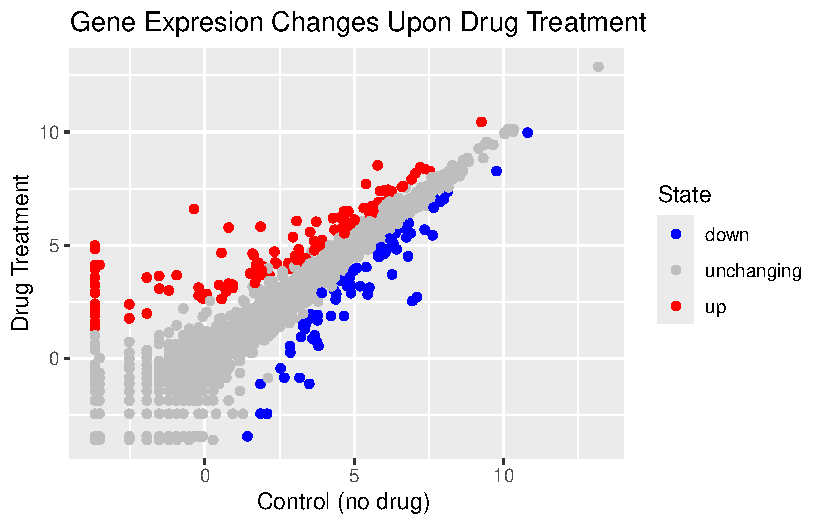
\includegraphics{class05_files/figure-pdf/unnamed-chunk-8-1.pdf}

\subsection{Running Code}\label{running-code}

When you click the \textbf{Render} button a document will be generated
that includes both content and the output of embedded code. You can
embed code like this:

\begin{Shaded}
\begin{Highlighting}[]
\DecValTok{1} \SpecialCharTok{+} \DecValTok{1}
\end{Highlighting}
\end{Shaded}

\begin{verbatim}
[1] 2
\end{verbatim}

You can add options to executable code like this

\begin{verbatim}
[1] 4
\end{verbatim}

The \texttt{echo:\ false} option disables the printing of code (only
output is displayed).




\end{document}
